\documentclass{article}

\usepackage[preprint]{neurips_2025}

\usepackage[utf8]{inputenc}
\usepackage[T1]{fontenc}
\usepackage{hyperref}
\usepackage{url}
\usepackage{booktabs}
\usepackage{graphicx}
\usepackage{amsmath}
\usepackage{microtype}
\usepackage{xcolor}

\title{Deep Reasoning via Cognitive Distillation and QLoRA}

\author{%
  Dimael Rivas\\
  \texttt{dimael.rivas@utec.edu.pe}
  \And
  Rodrigo Meza\\
  \texttt{rodrigo.meza@utec.edu.pe}
  \And
  Leonardo Candio\\
  \texttt{leonardo.candio@utec.edu.pe}
}

\begin{document}

\maketitle

\begin{abstract}
We build a compact mathematical-reasoning system that distills structured chain-of-thought behavior into a small open-weight language model. The pipeline generates supervised reasoning traces with explicit \texttt{<thinking>}, \texttt{<reflection>}, and \texttt{<answer>} regions, fine-tunes Qwen2.5-Instruct with 4-bit QLoRA adapters, and evaluates the resulting model against the base checkpoint on held-out GSM8K-style math problems. The final ablation focuses on Qwen2.5-1.5B-Instruct because the 3B model was less diagnostic for this dataset: its base behavior was already strong enough that improvements were harder to attribute. Our best adapter uses sequence length 1024, LoRA rank 8, alpha 16, learning rate $5\times10^{-5}$, and an effective batch size of 32. On a 30-problem screen it reached 63.3\% strict tagged accuracy with 90.0\% valid reasoning format. On a 100-problem confirmation set, it improved strict tagged-answer accuracy from 0.0\% to 48.0\% and valid format rate from 0.0\% to 75.0\%; however, under loose numeric answer extraction, the base model scored 55.0\% and the adapter scored 49.0\%. We conclude that cognitive distillation strongly teaches the requested reasoning protocol, but answer correctness remains sensitive to scoring protocol and incomplete generations.
\end{abstract}

\section{Introduction}
The project goal is to emulate part of the behavior of frontier reasoning systems---step-by-step planning, self-critique, and delayed final answers---using a model small enough to train with limited GPU time. Instead of changing the base architecture, we treat reasoning style as a supervised behavior to be distilled. A stronger teacher or prompt pipeline produces examples with explicit semantic regions:
\[
\texttt{<thinking>} \rightarrow \texttt{<reflection>} \rightarrow \texttt{<answer>}.
\]
The student model is then trained to reproduce this structure using supervised fine-tuning with low-rank adapters.

We use GSM8K-style grade-school math word problems as the target domain because they require multi-step symbolic reasoning while still allowing deterministic final-answer evaluation \citep{cobbe2021training}. The main research question is not only whether fine-tuning improves final numerical accuracy, but whether it reliably induces the desired reasoning protocol without making inference prohibitively expensive. This matters because test-time compute methods such as self-consistency can improve reasoning by sampling multiple solution paths, but they multiply latency and cost \citep{wang2022selfconsistency}.

The contributions are: (1) a reproducible data and QLoRA fine-tuning notebook; (2) a compact ablation over LoRA rank and learning rate; (3) a held-out comparison between the base and adapted model using paired examples; and (4) an analysis of the trade-off between structured reasoning behavior, answer accuracy, and inference latency.

\section{Approach}
\paragraph{Data distillation.}
The training data consists of approximately 2k GSM8K-style supervised examples stored as JSONL. Each target answer follows the same semantic template: a \texttt{<thinking>} section for the derivation, a \texttt{<reflection>} section for self-checking, and a \texttt{<answer>} section containing the final answer. This converts a normal math-answering task into a cognitive-distillation task: the model is not merely asked to produce the right number, but to imitate a reasoning procedure.

\paragraph{Model and parameter-efficient fine-tuning.}
We fine-tune Qwen2.5-1.5B-Instruct with QLoRA \citep{dettmers2023qlora}. The base model is loaded in 4-bit precision, while trainable LoRA adapters are inserted into attention and MLP projection matrices. This keeps the base weights frozen and trains only 9.23M--18.46M adapter parameters depending on rank. Table~\ref{tab:setup} summarizes the final training configuration.

\begin{table}[t]
\centering
\caption{Main training setup for the Qwen2.5-1.5B ablation.}
\label{tab:setup}
\resizebox{0.92\linewidth}{!}{\begin{tabular}{ll}
\toprule
Setting & Value \\ 
\midrule
Base model & Qwen2.5-1.5B-Instruct \\ 
Dataset & 2k distilled GSM8K-style reasoning traces \\ 
Sequence length & 1024 tokens \\ 
Quantization & 4-bit QLoRA, bfloat16 compute \\ 
LoRA target modules & q/k/v/o + gate/up/down projections \\ 
Batching & batch 8, grad. accumulation 4, effective 32 \\ 
Epoch budget & 3 epochs with early stopping monitor \\ 
Hardware & NVIDIA RTX PRO 6000 Blackwell Server Edition \\ 
\bottomrule
\end{tabular}
}
\end{table}

\paragraph{Inference-time scaling.}
The intended inference-time scaling mechanism is self-consistency: sample $N$ reasoning paths and select the most frequent semantic answer \citep{wang2022selfconsistency}. The implementation supports this procedure, but full $N=10$ evaluation was reserved for promising runs because early experiments showed that exhaustive sampling was too expensive for weak candidates. The final reported confirmation therefore uses paired greedy inference ($N=1$) over 100 held-out questions, while preserving the code path for majority voting in the notebook.

\section{Experiments}
All experiments were run on an NVIDIA RTX PRO 6000 Blackwell Server Edition. Training used sequence length 1024, batch size 8, gradient accumulation 4, bfloat16 compute, paged AdamW 8-bit, evaluation every 20 steps, and early-stopping monitoring. We tested three ablation settings:
\begin{itemize}
    \item rank 8, alpha 16, learning rate $5\times10^{-5}$;
    \item rank 8, alpha 16, learning rate $2\times10^{-5}$;
    \item rank 16, alpha 32, learning rate $5\times10^{-5}$.
\end{itemize}
Batch-size experiments with larger physical batches were attempted but recorded as out-of-memory cases, so batch 8 with accumulation was retained as the safe throughput setting. Each training run took roughly 9.2 minutes and used about 56 GiB peak allocated GPU memory.

Evaluation uses two complementary judges. The strict judge requires a parseable answer inside the requested tag structure, so it directly measures obedience to the project protocol. The loose numeric judge extracts the final number even if the response does not satisfy the tag format; this better approximates raw math-answering ability. We report both because they answer different questions.

\section{Results}

\begin{table}[t]
\centering
\caption{Fast 30-problem ablation screen. Accuracy, format, and reflection are percentages.}
\label{tab:ablation}
\resizebox{\linewidth}{!}{\begin{tabular}{lrrrrrrr}
\toprule
Configuration & LoRA r & LR & Eval loss & Acc. 30 & Format & Reflect. & Time (min) \\ 
\midrule
r=8, lr=5e-5 & 8 & 5e-05 & 0.402 & 63.3 & 90.0 & 90.0 & 9.2 \\ 
r=8, lr=2e-5 & 8 & 2e-05 & 0.456 & 56.7 & 80.0 & 80.0 & 9.2 \\ 
r=16, lr=5e-5 & 16 & 5e-05 & 0.383 & 53.3 & 80.0 & 83.3 & 9.2 \\ 
\bottomrule
\end{tabular}
}
\end{table}

\begin{figure}[t]
\centering
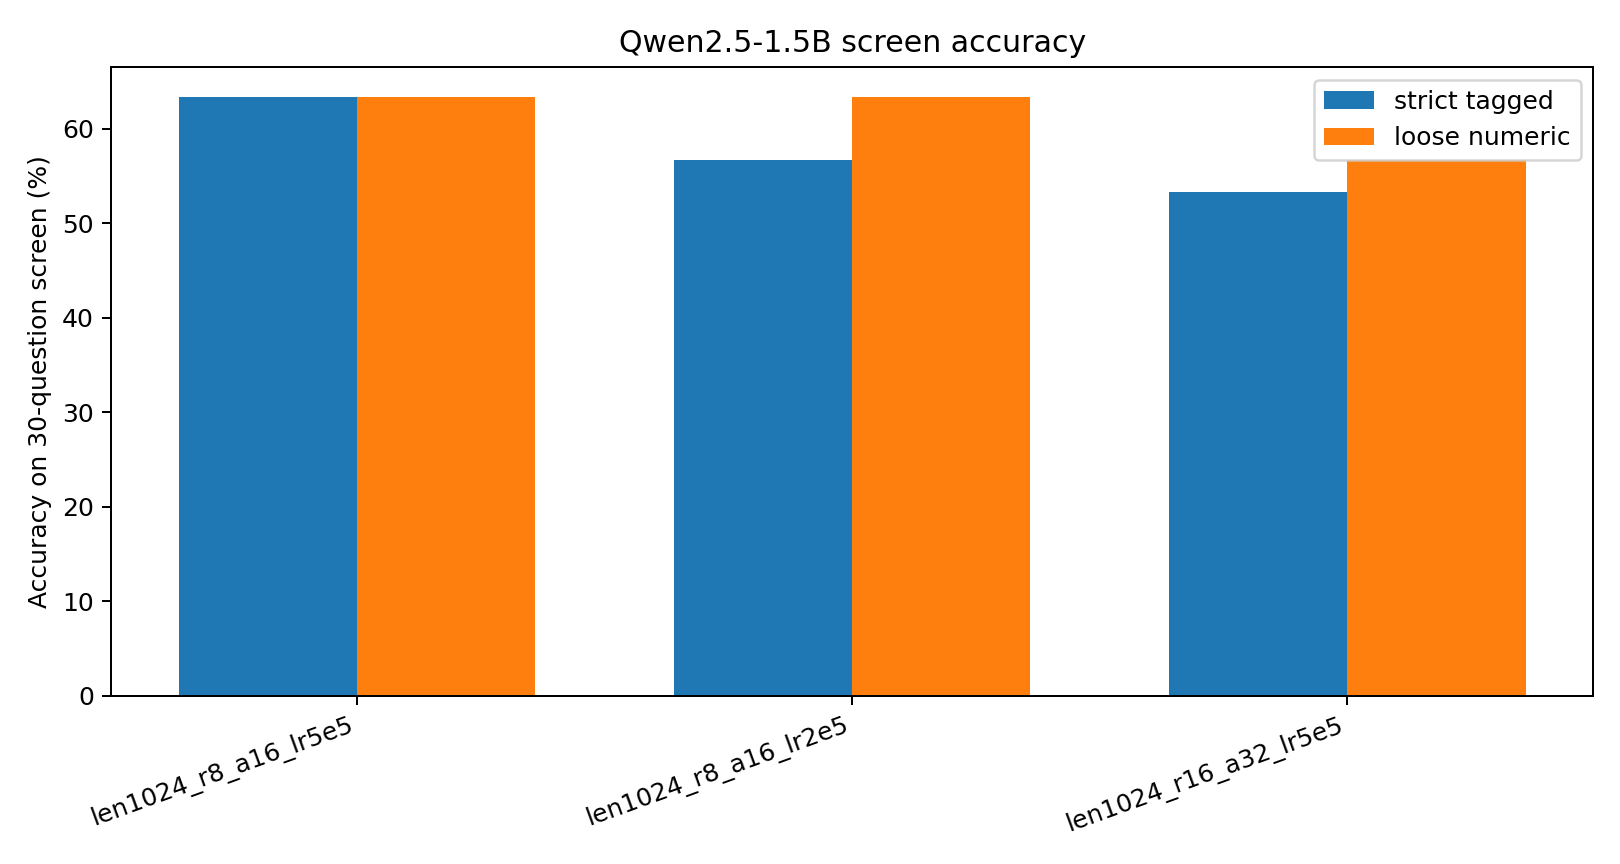
\includegraphics[width=0.48\linewidth]{figures/screen_accuracy.png}
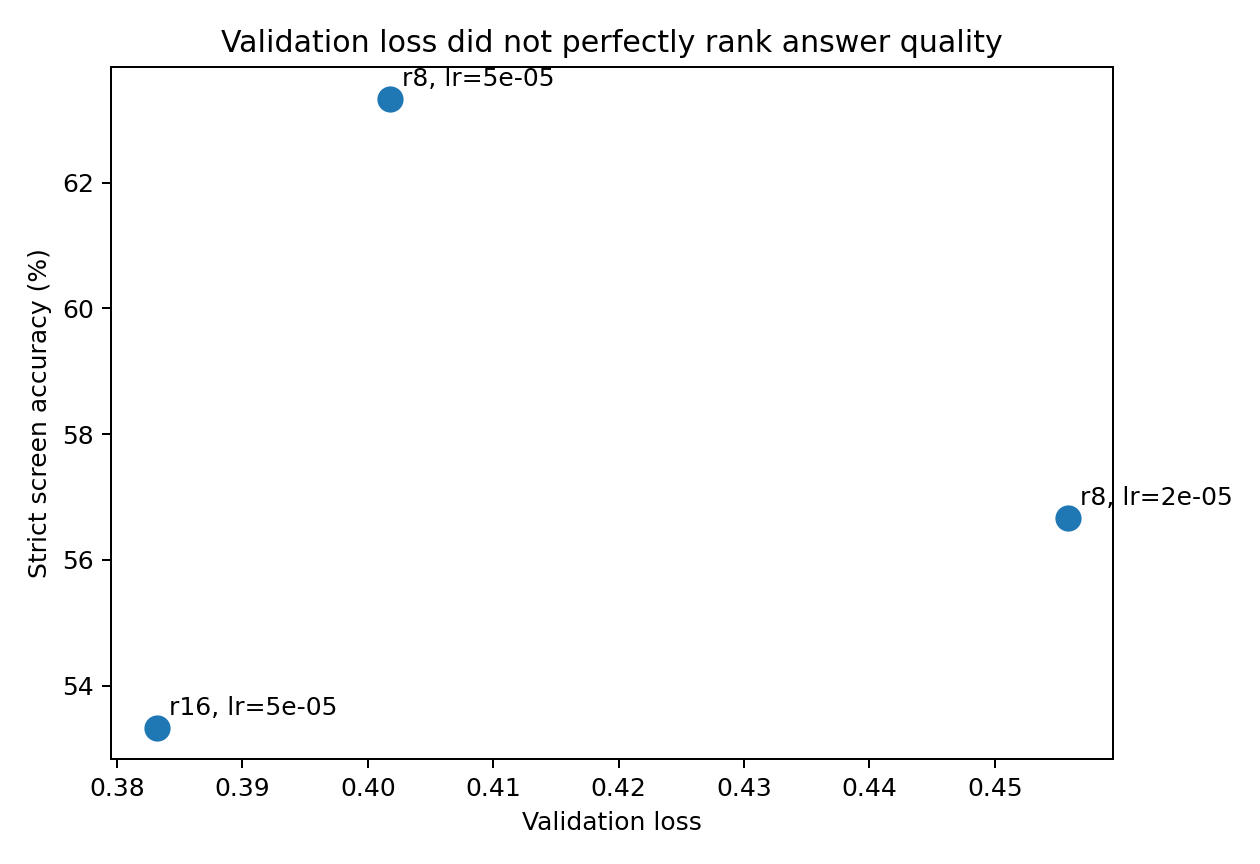
\includegraphics[width=0.48\linewidth]{figures/loss_vs_accuracy.png}
\caption{Left: fast-screen strict accuracy for the ablation. Right: validation loss was not a perfect proxy for final-answer accuracy; the rank-16 model had the lowest validation loss but worse answer accuracy than rank 8.}
\label{fig:screen}
\end{figure}

Table~\ref{tab:ablation} and Figure~\ref{fig:screen} show that the best fast-screen configuration was rank 8, alpha 16, and learning rate $5\times10^{-5}$. It reached 63.3\% strict tagged accuracy, 90.0\% valid format rate, and 90.0\% reflection rate on 30 held-out problems. The lower learning rate matched its loose accuracy but produced weaker strict formatting. Increasing rank to 16 reduced answer accuracy despite lowering validation loss, suggesting that imitation loss alone did not fully predict robust mathematical correctness.

\begin{figure}[t]
\centering
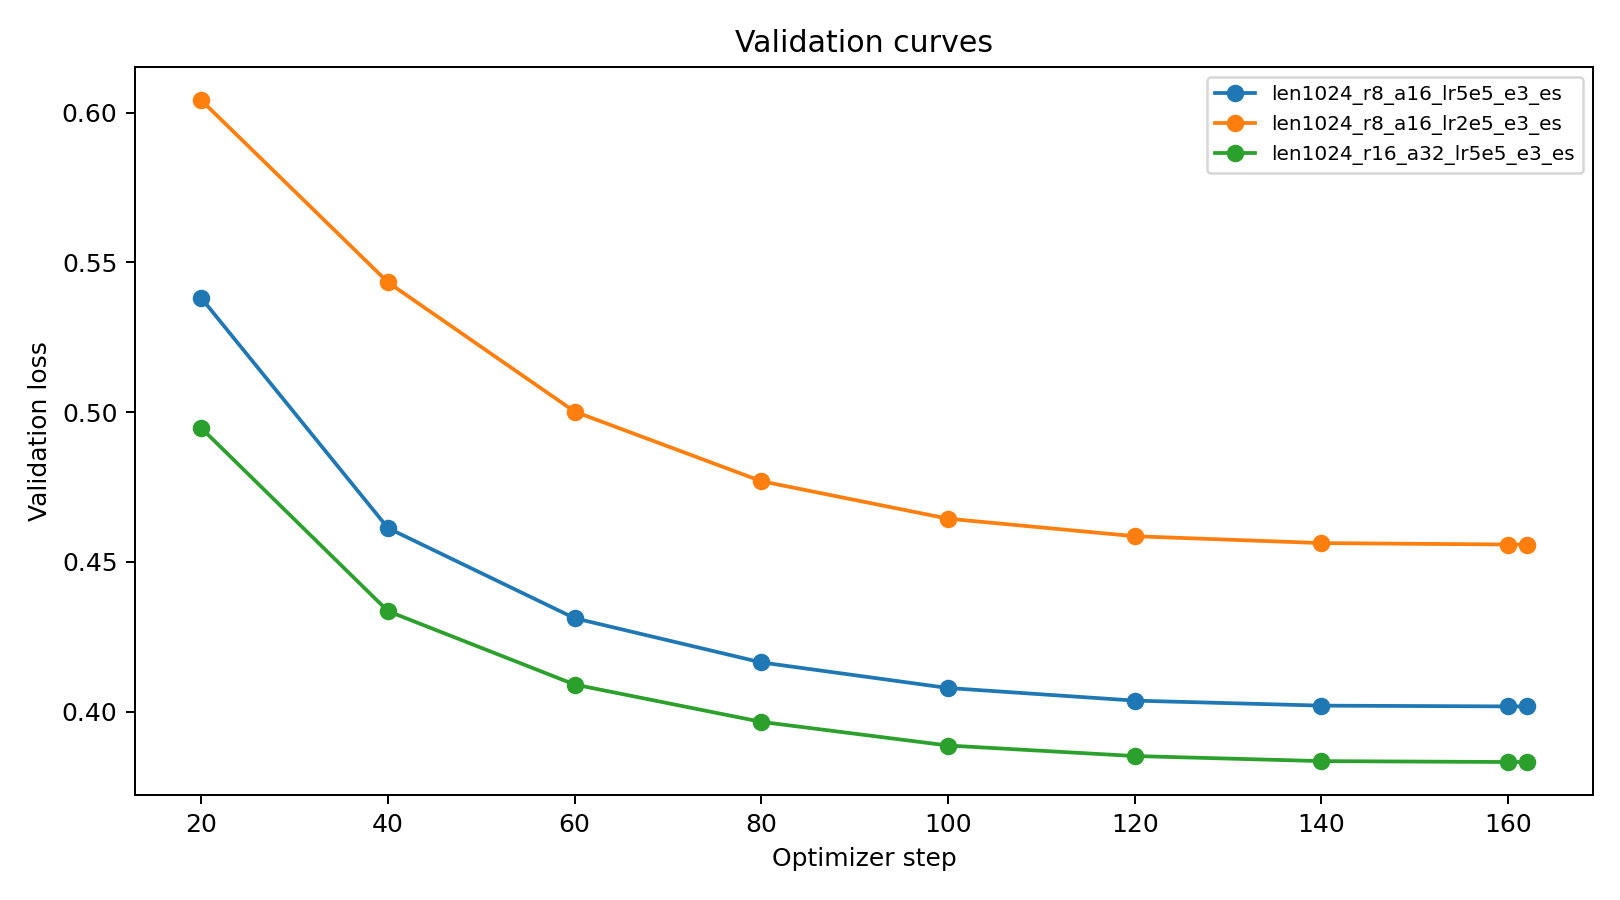
\includegraphics[width=0.70\linewidth]{figures/validation_curves.png}
\caption{Validation loss curves for the QLoRA ablation. All runs trained stably, but the best validation loss did not correspond to the best held-out answer accuracy.}
\label{fig:validation}
\end{figure}

\begin{table}[t]
\centering
\caption{Held-out 100-problem confirmation for the selected adapter. Values are percentages except latency.}
\label{tab:confirm}
\resizebox{\linewidth}{!}{\begin{tabular}{lrrrr}
\toprule
Metric & Base & Adapter & Delta & 95\% bootstrap CI \\ 
\midrule
Strict tagged answer acc. & 0.0 & 48.0 & +48.0 & [+38.0, +58.0] \\ 
Loose numeric answer acc. & 55.0 & 49.0 & -6.0 & [-19.0, +6.0] \\ 
Valid format rate & 0.0 & 75.0 & +75.0 & -- \\ 
Reflection rate & 0.0 & 75.0 & +75.0 & -- \\ 
Latency (s/sample) & 4.19 & 15.69 & +11.49 & -- \\ 
\bottomrule
\end{tabular}
}
\end{table}

\begin{figure}[t]
\centering
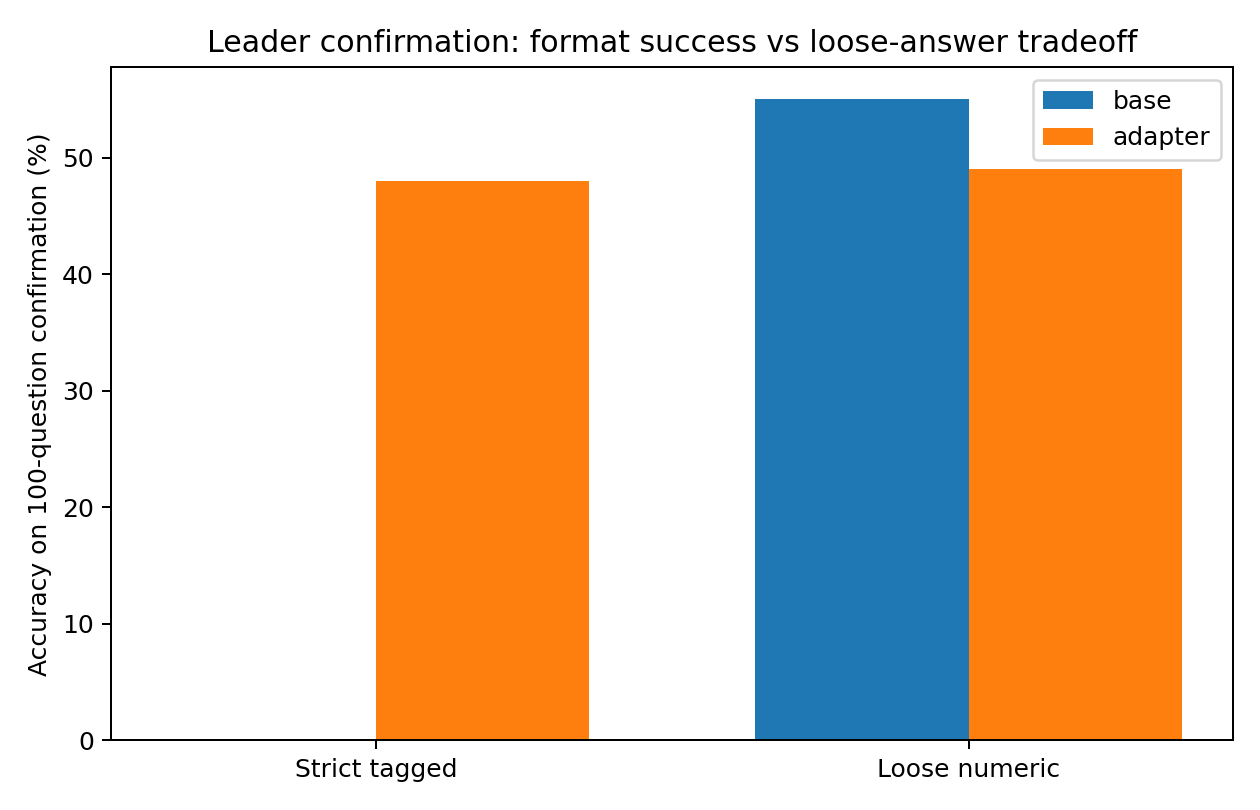
\includegraphics[width=0.48\linewidth]{figures/confirm_accuracy.png}
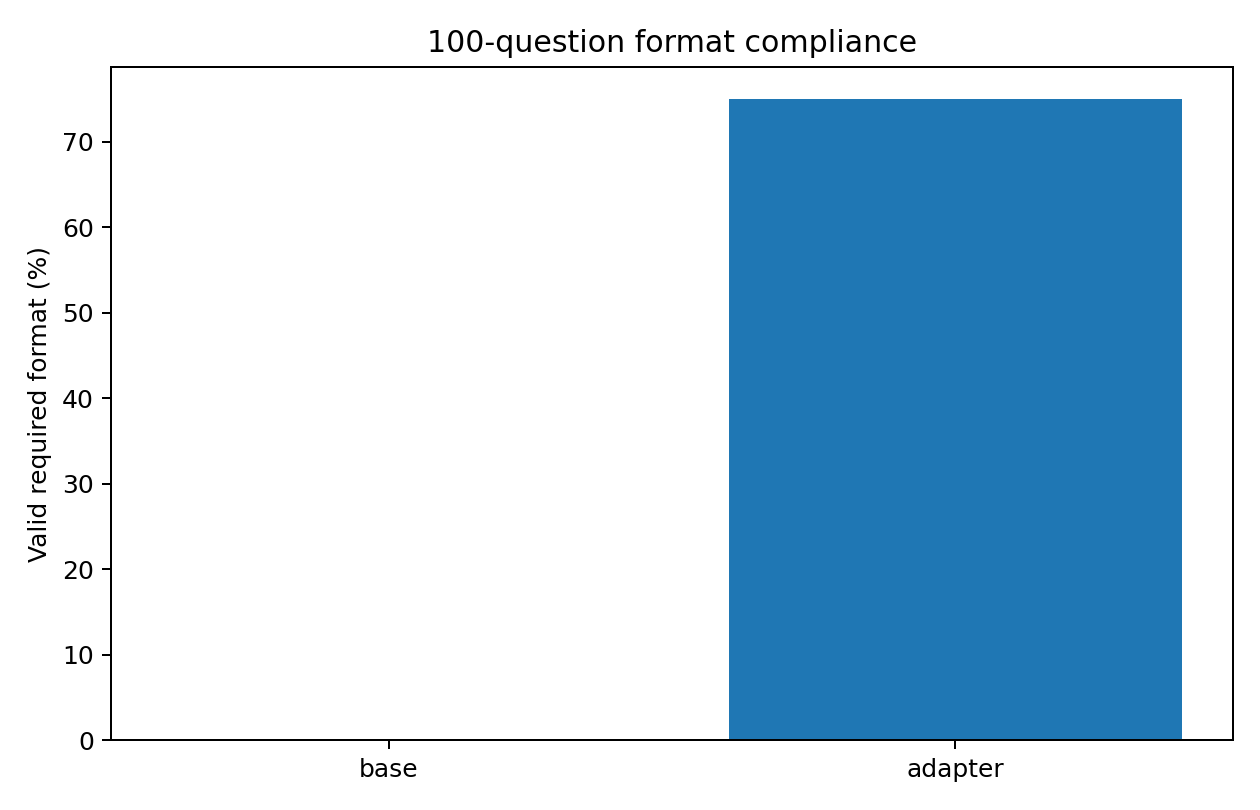
\includegraphics[width=0.48\linewidth]{figures/confirm_format_rate.png}
\caption{Held-out confirmation. The adapter strongly improves strict protocol-following metrics, but loose numeric accuracy remains competitive for the base model.}
\label{fig:confirm}
\end{figure}

The 100-problem confirmation in Table~\ref{tab:confirm} clarifies the trade-off. The base model almost never emits the required tags, so its strict tagged-answer accuracy is 0.0\%. The adapter raises strict accuracy to 48.0\% and valid format/reflection rates to 75.0\%. This is the clearest success of the project: the fine-tuned model learns to externalize a structured reasoning trace.

However, loose numeric scoring tells a more conservative story. The base model reaches 55.0\% loose numeric accuracy, while the adapter reaches 49.0\%; the paired bootstrap interval for the adapter-base difference is $[-19,+6]$ percentage points. Therefore, the adapter should not be claimed to dominate the base model in raw math accuracy. It is better described as a protocol-aligned reasoning model whose answer accuracy is close to, but not reliably above, the original checkpoint.

\section{Analysis}
\paragraph{Why the 1.5B model became the main study.}
The project description originally targets a model around 3B parameters. In practice, Qwen2.5-3B-Instruct was strong enough on the selected GSM8K-style problems that the dataset did not expose a clear weakness. We therefore repeated the same training and evaluation pipeline with Qwen2.5-1.5B-Instruct. This made the distillation effect more visible and produced a more meaningful ablation: the student was small enough to struggle, but still capable of learning the reasoning format.

\paragraph{Protocol learning versus mathematical learning.}
The largest gain is in structure. The adapter learns when to think, when to reflect, and where to put the answer. This is useful for interpretability and for downstream judges that expect explicit sections. Yet the loose numeric result shows that structure alone is not sufficient. Some generations contain long reasoning traces but fail to terminate cleanly or introduce algebraic mistakes during reflection. The live notebook inference example intentionally illustrates this: a model can produce a plausible trace and still end with the wrong number.

\paragraph{Validation loss is not enough.}
The rank-16 configuration obtained the lowest validation loss (0.383) but underperformed the rank-8 learning-rate-$5\times10^{-5}$ run on strict answer accuracy. A likely explanation is that token-level imitation loss rewards matching the teacher style, including long explanations, while final-answer accuracy depends on brittle arithmetic steps and clean completion. For this task, validation loss should be treated as a stability signal, not the only model-selection criterion.

\paragraph{Test-time compute trade-off.}
Self-consistency remains the natural next step: sample multiple traces, extract the final answer from each, and vote. It is especially attractive here because the adapter often produces well-formed traces, which makes semantic answer extraction easier. The cost is latency. Greedy adapter inference already averages 15.69 seconds per sample versus 4.19 seconds for the base model. Running $N=10$ self-consistency naively would be roughly an order of magnitude slower, so it should be reserved for problems where accuracy matters more than throughput.

\section{Conclusion}
QLoRA-based cognitive distillation successfully taught a compact Qwen2.5 model to emit explicit reasoning, reflection, and answer tags. The best configuration was LoRA rank 8, alpha 16, learning rate $5\times10^{-5}$, sequence length 1024, and effective batch size 32. It achieved the strongest fast-screen result and improved strict protocol-aware held-out accuracy from 0.0\% to 48.0\%. At the same time, the base model remained slightly stronger under loose numeric scoring, 55.0\% versus 49.0\%, so the final conclusion is not that fine-tuning universally improves mathematical accuracy. The defensible conclusion is that supervised cognitive distillation makes the model substantially more judgeable and protocol-compliant, while further work is needed to convert that structure into reliable numerical gains.

Future work should run multi-seed evaluations, expand the distilled dataset, use stronger filtering for teacher traces, evaluate a true external LLM-as-a-judge rubric for logical rigor and self-correction, and selectively apply self-consistency to the best adapter under a fixed latency budget.

\clearpage
\bibliographystyle{plainnat}
\bibliography{references}

\end{document}
